%#########################################################################
\chapter{Electrostática}
\label{cha:electrostatic}

La electrostática estudia la interacción entre cuerpos cargados 
eléctricamente sin tener en cuenta su movimiento. Esta simplificación 
permite ignorar términos dinámicos asociados a corrientes eléctricas y 
campos magnéticos inducidos.

\

En este capítulo se realizan algunas demostraciones computacionales que 
van desde el cálculo de trayectorias de partículas en campos eléctricos y 
magnéticos, la representación de las líneas de campo y superficies 
equipotenciales de distribuciones de carga, hasta el cálculo de 
capacitancia de algunos sistemas.
%#########################################################################



\
%*************************************************************************
\section{Demostración 1: Espectrómetro de Masas}
\label{sec:DEMO2_01}
\rule{14cm}{0.5mm}

En esta primera demostración será estudiado el espectrómetro de masas. El 
objetivo de este dispositivo es caracterizar partículas cargadas de acuerdo
a su relación carga masa $(q/m)$. Su funcionamiento consiste en la inmersión 
de las partículas en un campo magnético o eléctrico (este caso) y a partir de
las trayectorias obtenidas determinar su relación carga masa (ver figura 
\ref{fig:mass_spectrometer}).

\

Tomando una partícula de masa $m$ y carga $q$ embebida en un campo eléctrico
homogéneo y uniforme $\bds E$, la ecuación de movimiento es


%.........................................................................
%Movement equation
\eq{eq:charged_particle}
{m\dtot{^2\bds r}{t^2} = q\bds E}
%.........................................................................


Tomando el sistema coordenado de tal forma que el campo $\bds E$ esté en la
dirección positiva de y, se obtiene


%.........................................................................
%Mass Spectrometer
\begin{figure}[htbp]
	\centering
	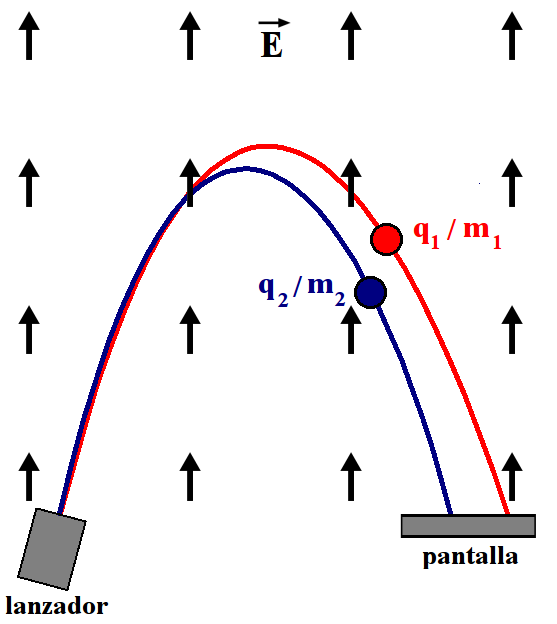
\includegraphics[width=0.50\textwidth]
	{./pictures/mass_spectrometer.png}

	\caption{\small{Espectrómetro de masas.}}
	
	\label{fig:mass_spectrometer}
\end{figure}
%.........................................................................


%.........................................................................
%Movement equations solution
\begin{eqnarray}
\label{eq:x_equation}
x(t) &=& x_0 + v_{x0}t \\
\label{eq:y_equation}
y(t) &=& y_0 + v_{y0}t + \frac{1}{2}\pr{\frac{q}{m}}t^2
\end{eqnarray}
%.........................................................................
donde se ha introducido la posición inicial de la partícula $\bds r(t=0) = 
(x_0, y_0)$ y la velocidad inicial $\bds v(t=0) = (v_{x0}, v_{y0})$.

\

Eliminando el tiempo de las dos ecuaciones se obtiene la siguiente 
trayectoria


%.........................................................................
%Trayectory
\eq{eq:trayectory}
{y(x) = y_0 + \frac{v_{y0}}{v_{x0}}(x - x_0) + 
\frac{1}{2}\pr{\frac{q}{m}} \pr{ \frac{x - x_0}{v_{x0}} }^2}
%.........................................................................

\

En el siguiente código de \python se grafica la trayectoria de dos 
partículas con diferente relación carga masa. La primera tiene una 
relación $q_1/m_1 = -1\mbox{ C}/1 \mbox{ kg}$ y la segunda $q_2/m_2 = 
-1\mbox{ C}/2 \mbox{ kg}$. Ambas partículas se disparan del origen y con 
una elocidad inicial de $\bds v_0 = (1, 2) \mbox{ m/s}$. El campo eléctrico 
tiene una intensidad de $|\bds E| = 1 \mbox{ N/C}$.

\newpage
%ccccccccccccccccccccccccccccccccccccccccccccccccccccccccccccccccccccccccc
%DEMO 2_01
\begin{listing}[style=python]
#!/usr/bin/env python
#==========================================================
# DEMOSTRACION 1
# Espectrometro de masas
#==========================================================
from __future__ import division
import numpy as np
import matplotlib.pylab as plt

#Trayectoria
def trayectory(x):
    y = y0 + vy0/vx0*(x - x0) + 0.5*(q/m)*( (x-x0)/vx0 )**2
    return y
    
#PARTICULA 1
#Carga
q = -1
#Masa
m = 1
#Posicion inicial
x0 = 0
y0 = 0
#Velocidad inicial
vx0 = 1
vy0 = 2
#Valores de X a graficar
X = np.arange( 0, 10, 0.01 )
#Trayectoria
Y = trayectory( X )
#Grafica de trayectoria
plt.plot( X, Y, label='particula 1' )

#PARTICULA 2
#Carga
q = -1
#Masa
m = 2
#Posicion inicial
x0 = 0
y0 = 0
#Velocidad inicial
vx0 = 1
vy0 = 2
#Valores de X a graficar
X = np.arange( 0, 10, 0.01 )
#Trayectoria
Y = trayectory( X )
#Grafica de trayectoria
plt.plot( X, Y, label='particula 2' )

#Limites del eje X
plt.xlim( (0,10) )
#Limites del eje Y
plt.ylim( (0,10) )
plt.legend()
plt.show()
\end{listing}
%ccccccccccccccccccccccccccccccccccccccccccccccccccccccccccccccccccccccccc


El resultado que se obtiene es


%.........................................................................
%Trayectories
\begin{figure}[htbp]
	\centering
	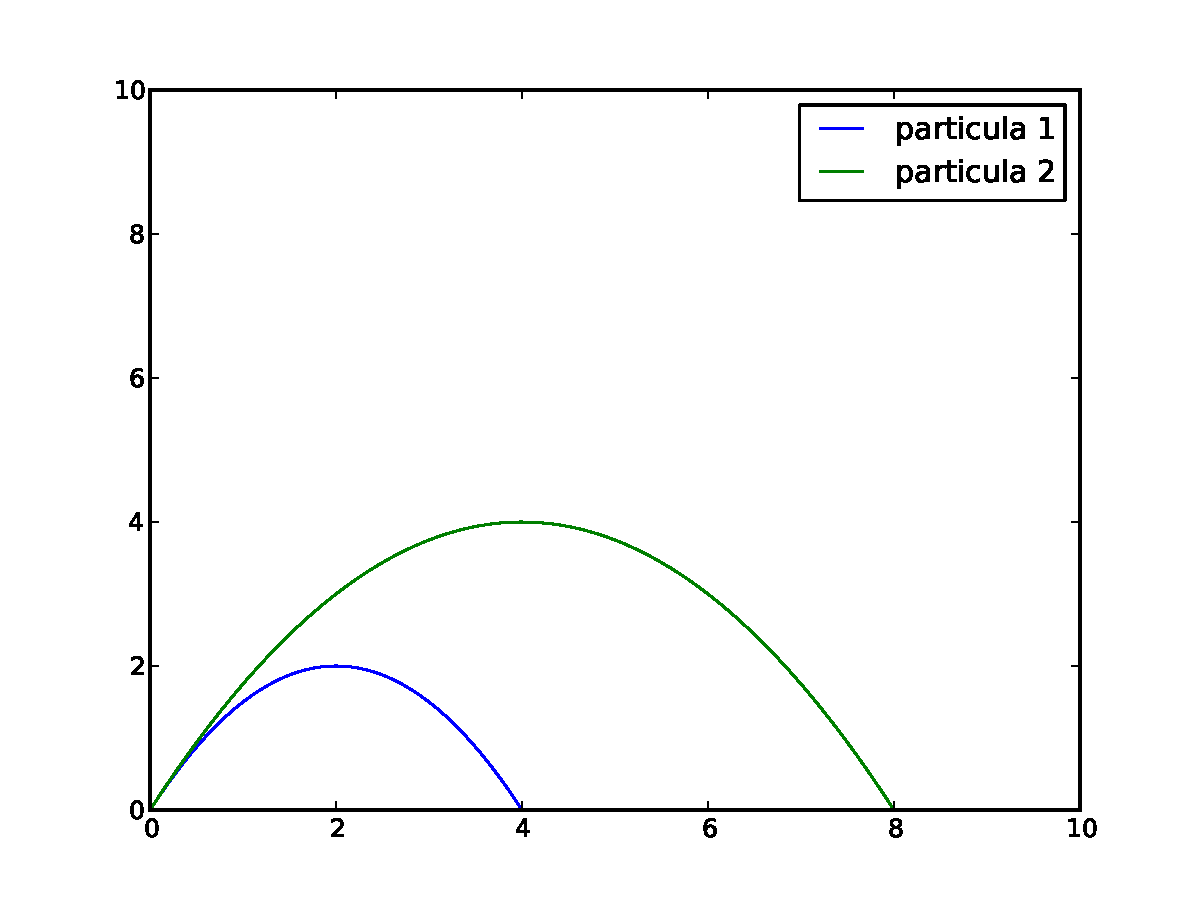
\includegraphics[width=0.8\textwidth]
	{./pictures/demo2_01.pdf}

	\caption{\small{Trayectorias según la relación carga masa de las 
	partículas.}}
	
	\label{fig:trayectories}
\end{figure}
%.........................................................................


La representación de la trayectoria de forma gráfica permite entonces 
comparar directamente con datos medidos en un laboratorio, por ejemplo 
trayectorias de partículas en cámaras de burbujas.

\newpage

A continuación se explica cada componente del código anterior


%ccccccccccccccccccccccccccccccccccccccccccccccccccccccccccccccccccccccccc
%DEMO 2_01
\begin{listing}[style=python, numbers = none]
from __future__ import division
import numpy as np
import matplotlib.pylab as plt
\end{listing}
%ccccccccccccccccccccccccccccccccccccccccccccccccccccccccccccccccccccccccc
En la primera línea se carga el módulo \texttt{division}, este permite a 
\python calcular fracciones de números enteros como cantidades reales. En
la siguiente línea se carga la librería \numpy con el alias de \texttt{np}
y finalmente se carga la librería \matplotlib con el alias de \texttt{plt}.


%ccccccccccccccccccccccccccccccccccccccccccccccccccccccccccccccccccccccccc
%DEMO 2_01
\begin{listing}[style=python, numbers = none]
#Trayectoria
def trayectory(x):
    y = y0 + vy0/vx0*(x - x0) + 0.5*(q/m)*( (x-x0)/vx0 )**2
    return y
\end{listing}
%ccccccccccccccccccccccccccccccccccccccccccccccccccccccccccccccccccccccccc
En esta parte se define la trayectoria de la partícula en el campo 
eléctrico descrito.

%ccccccccccccccccccccccccccccccccccccccccccccccccccccccccccccccccccccccccc
%DEMO 2_01
\begin{listing}[style=python, numbers = none]    
#PARTICULA 1
#Carga
q = -1
#Masa
m = 1
#Posicion inicial
x0 = 0
y0 = 0
#Velocidad inicial
vx0 = 1
vy0 = 2
#Valores de X a graficar
X = np.arange( 0, 10, 0.01 )
#Trayectoria
Y = trayectory( X )
#Grafica de trayectoria
plt.plot( X, Y, label='particula 1' )
\end{listing}
%ccccccccccccccccccccccccccccccccccccccccccccccccccccccccccccccccccccccccc
Se definen las propiedades físicas y cinemáticas de la partícula 1. Su 
carga, su masa, su posición y velocidad inicial. Luego, usando el comando
\texttt{arange} de la librería \numpy, se construye un arreglo de valores 
en el eje X que serán usados para el cálculo de la trayectoria. En este 
caso se toma desde 0 a $10$ m con un salto de $0.01$ m. Finalmente se 
llama la función de la trayectoria de la partícula en todos los valores de
\texttt{X} y se grafica, usando como etiqueta \texttt{label='particula 1'}.


%ccccccccccccccccccccccccccccccccccccccccccccccccccccccccccccccccccccccccc
%DEMO 2_01
\begin{listing}[style=python, numbers = none]
#Limites del eje X
plt.xlim( (0,10) )
#Limites del eje Y
plt.ylim( (0,10) )
plt.legend()
plt.show()
\end{listing}
%ccccccccccccccccccccccccccccccccccccccccccccccccccccccccccccccccccccccccc
Finalmente se usan las funciones de \matplotlib \texttt{xlim} y \texttt{ylim}
para fijar los límites de la ventana de graficación. La función 
\texttt{legend} muestra las etiquetas de las dos trayectorias y finalmente
\texttt{show} muestra en pantalla el resultado.


\rule{14cm}{0.5mm}
%*************************************************************************